%# -*- coding: utf-8-unix -*-

\chapter{结合共享账户的机票推荐算法}
\label{chap:share}

本章我们研究机票推荐中的共享账户问题,该问题主要针对一个用户ID包括多个乘客的情况。我们将提出一种算法,可以预测出用户下本次购票的乘客的概率分布,从而学习更具针对性的偏好模型,提升推荐准确率。

\section{机票推荐中的共享账户}

推荐算法总体分为两类,一类是根据用户和物品之间的关系,提出衡量用户相似度以及物品相似度的算法,为用户根据物品或用户之间的相似度提供推荐结果;另一类是基于内容的推荐,物品可以表示为特征的集合(包括显性特征和隐性特征),从用户的物品列表中学习用户对每个特征的偏好。为用户推荐最符合其特征偏好的物品。

以这两类算法为代表的传统推荐系统通常以用户在网站的注册ID(账户)来识别用户,它们一般假定一个用户背后只有一个使用者,即每个用户仅包含一个固定的偏好模型。然而在很多领域,都会发生现实中几个人共同使用一个账户的情景。例如,在购物网站,可能一个家庭共用一个账户,每位家庭成员都可以使用这个账户进行购物;在一般的线旅行票务服务网站,例如机票、酒店、旅游等业务领域,一个账户中也可能会有几个成员,他们可能会为家人、旅伴购票。


第一种情形中,虽然会有几位家庭成员共同使用账户购物,但是服务商无法获取购物者的真实身份信息。而对于第二种情形,如图\ref{fig:fill_id}所示,乘客在订票后会被要求填写身份信息,因此,网站可以获取其真实身份。在机票数据集中,订单包含了每一位乘客的身份信息,包括姓名、性别、年龄、证件号码等。在我们进行数据分析与实验过程中,统一使用加密后的证件号码来代指乘客,既确保了乘客之间无冲突,又保护了乘客隐私。

\begin{figure}
 \centering
 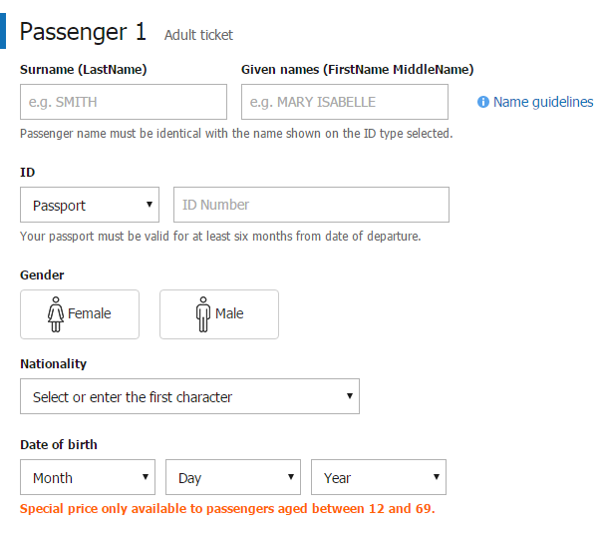
\includegraphics[width=0.75\linewidth]{05/1_fill_id.png}
 \bicaption[fig:fill_id]{填写乘客信息}{用户在票务网站填写身份信息}{Fig}{Users Fill in Their Identification on Website}
\end{figure}

通常来说,同一个用户下乘客可能具有较为相似的偏好,但他们之间的差异也不能忽视。如果我们能够利用购票时获取的乘客身份信息为该乘客进行机票推荐,就可以为每位乘客建立特征分布模型,更具针对性的细粒度乘客模型对进一步提升个性化机票推荐准确率可以起到作用。然而,按照业务流程,只有当用户选定机票后才会填写身份信息。在我们进行机票推荐时还无法获取乘客信息。我们需要预测乘客的概率分布。

我们的问题是在共享账户的乘客选购机票时,根据乘客历史行为模式以及当前会话的上下文预测出当前是哪几位乘客在网站登录。

\section{乘客预测模型}

\section{结合乘客预测的机票个性化推荐}

\section{实验结果分析}